\documentclass[text05.tex]{subfiles}
\begin{document}
\subsubsection{ボリューム}\label{volume}
\begin{table}[H]
  \begin{widerrows}
    \begin{tabular}{|p{\colF}|p{\colG}|}	\hline
    \ruby{名称}{めい|しょう} & ボリューム（ぼりゅーむ）\\ \hline
    \ruby{接続箇所}{せつ|ぞく|か|しょ} & アナログコネクタ (3pin)\\ \hline
    \ruby{機能概要}{き|のう|がい|よう} & つまみの回転量を出力\\ \hline
    \end{tabular}
  \end{widerrows} 
\end{table}

\begin{table}[H]
  \begin{widerrows}
    \begin{tabular}{|p{\colF}|p{\colG}|}	\hline
    サンプルコードの場所 & 05/anain.hsp\\ \hline
    raspiへの入力 & つまみの回転量 0から1023の\ruby{値}{あたい}\\ \hline
    raspiへの入力方法 & val = \adcget(ピン番号, チャンネル番号)\\ \hline
    raspiからの出力 & なし\\ \hline
    raspiからの出力方法 & なし\\ \hline
    \end{tabular}
  \end{widerrows} 
\end{table}

\begin{figure}[H]
  \begin{widerrows}
    \begin{tabular}{|p{\colF}|p{\colG}|} \hline
    使い道 & 音量調整, LEDの明るさ調整, ゲームのコントローラとして\\ \hline
    \ruby{注意事項}{ちゅう|い|じ|こう} & 強く\ruby{押}{お}して\ruby{壊}{こわ}さないように注意\\ \hline
    \ruby{補足}{ほ|そく} & \ruby{先端}{せん|たん}のつまみをつまんで回転させると\ruby{抵抗値}{てい|こう|ち}が変化しraspberry piに入力される\ruby{電圧}{でん|あつ}が変化します。今回使うボリュームは左に回しきったときは変化が小さく、右に回すほど変化が大きくなります（指数関数的）。この\ruby{設定}{せっ|てい}をAカーブと\ruby{呼}{よ}びます (図\ref{ボリュームの特性})。これはボリュームがしばしば音量調節に利用され、人間の耳の感度は対数関数的（小さい音ほど\ruby{敏感}{びん|かん}で大きい音に関しては\ruby{鈍感}{どん|かん}）であることからこのように\ruby{設定}{せっ|てい}されています。もちろん、ボリュームは音量調節以外にも使用されるため、\ruby{用途}{よう|と}に\ruby{応}{おう}じて\ruby{特性}{とく|せい}が線形(\ruby{傾}{かたむ}きが一定)なBカーブや対数関数的（\ruby{傾}{かたむ}きが小さくなっていく）なCカーブなどが\ruby{存在}{そん|ざい}します。このパーツは A カーブです。\par
  ボリュームには\ruby{端子}{たん|し}が3つ付いており、図\ref{ボリュームの仕組み}のように１つに+\ruby{電源}{でん|げん}を、１つに-\ruby{電源}{でん|げん}をつなげ、もう１つを出力として使用します。+\ruby{電源}{でん|げん}から-\ruby{電源}{でん|げん}までに\ruby{帯状}{おび|じょう}の\ruby{抵抗器}{てい|こう|き}が\ruby{接続}{せつ|ぞく}されており、その間に出力の\ruby{端子}{たん|し}が\ruby{接続}{せつ|ぞく}されています。シャフトを回すことで、出力\ruby{端子}{たん|し}の位置が変化し、結果プラス\ruby{電源}{でん|げん}\ruby{端子}{たん|し}-出力\ruby{端子}{たん|し}間と出力\ruby{端子}{たん|し}-マイナス\ruby{電源}{でん|げん}\ruby{端子}{たん|し}間の\ruby{抵抗値}{てい|こう|ち}が変化することになります。

    \begin{minipage}[t][7.0cm][t]{0.48\linewidth}
      \begin{minipage}[c][4.8cm][c]{\linewidth}
        \centering
        \includesvg[width=\linewidth,keepaspectratio]{../../asset/image/volume_curves.svg}
      \end{minipage}
      \caption{ボリュームの\ruby{特性}{とく|せい}\hspace{0pt}}
      \label{ボリュームの特性}
    \end{minipage}%
    \hfill
    \begin{minipage}[t][7.0cm][t]{0.48\linewidth}
      \begin{minipage}[c][4.8cm][c]{\linewidth}
        \centering
        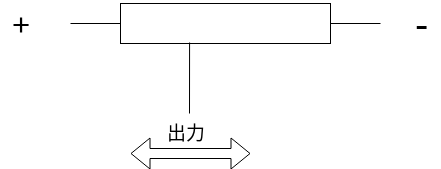
\includegraphics[width=\linewidth,keepaspectratio]{../../asset/image/text05-img051.png}
      \end{minipage}
      \caption{ボリュームの仕組み}
      \label{ボリュームの仕組み}
    \end{minipage}\\ \hline
    \end{tabular}
  \end{widerrows} 
\end{figure}

\begin{figure}[H]
  \begin{widerrows}
    \begin{tabular}{|p{\colH}|p{\colI}|p{\colH}|p{\colI}|} \hline
    外観 & 
    \begin{minipage}[t]{\linewidth}
      \smallskip
        \centering
        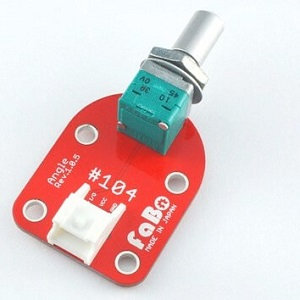
\includegraphics[width=0.5\linewidth]{../../asset/image/text05-img022.jpg}
        \caption{ボリューム}
        \smallskip
      \end{minipage} &
      回路記号 & 
      \begin{minipage}[t]{\linewidth}
      \smallskip
        \centering
        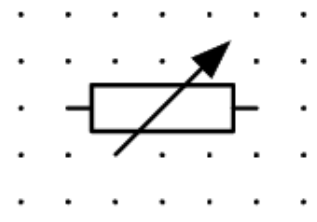
\includegraphics[width=0.5\linewidth]{../../asset/image/text05-img052.png}
        \caption{ボリュームの回路図}
        \smallskip
      \end{minipage}\\ \hline
    \end{tabular}
  \end{widerrows} 
\end{figure}\end{document}
